\documentclass{article}
\usepackage{graphicx} % Required for inserting images
\usepackage{listings}
\usepackage{hyperref}
\documentclass{article}
\usepackage{graphicx} % Required for including images


\title{101 Final Project Checkpoint}
\author{Kartikeya Sharma, Clement Lui, Richard Villagomez, Nicholas Chae}
\date{\today}

\begin{document}

\maketitle

\section{Dataset Description}

We selected the \href{https://www.yelp.com/dataset}{Yelp Open Dataset}, a 8.65 GB dataset which contains a subset of businesses, user data, and reviews provided as JSON files. The dataset is made up of 6,990,280 reviews, 150,346 businesses, and 200,100 pictures (not utilized in our project) from 11 metropolitan areas. Over 1.2 million business attributes are accessible along with 908,915 tips (quick suggestions) from 1,987,897 users.

\begin{figure}[h!]
    \centering
    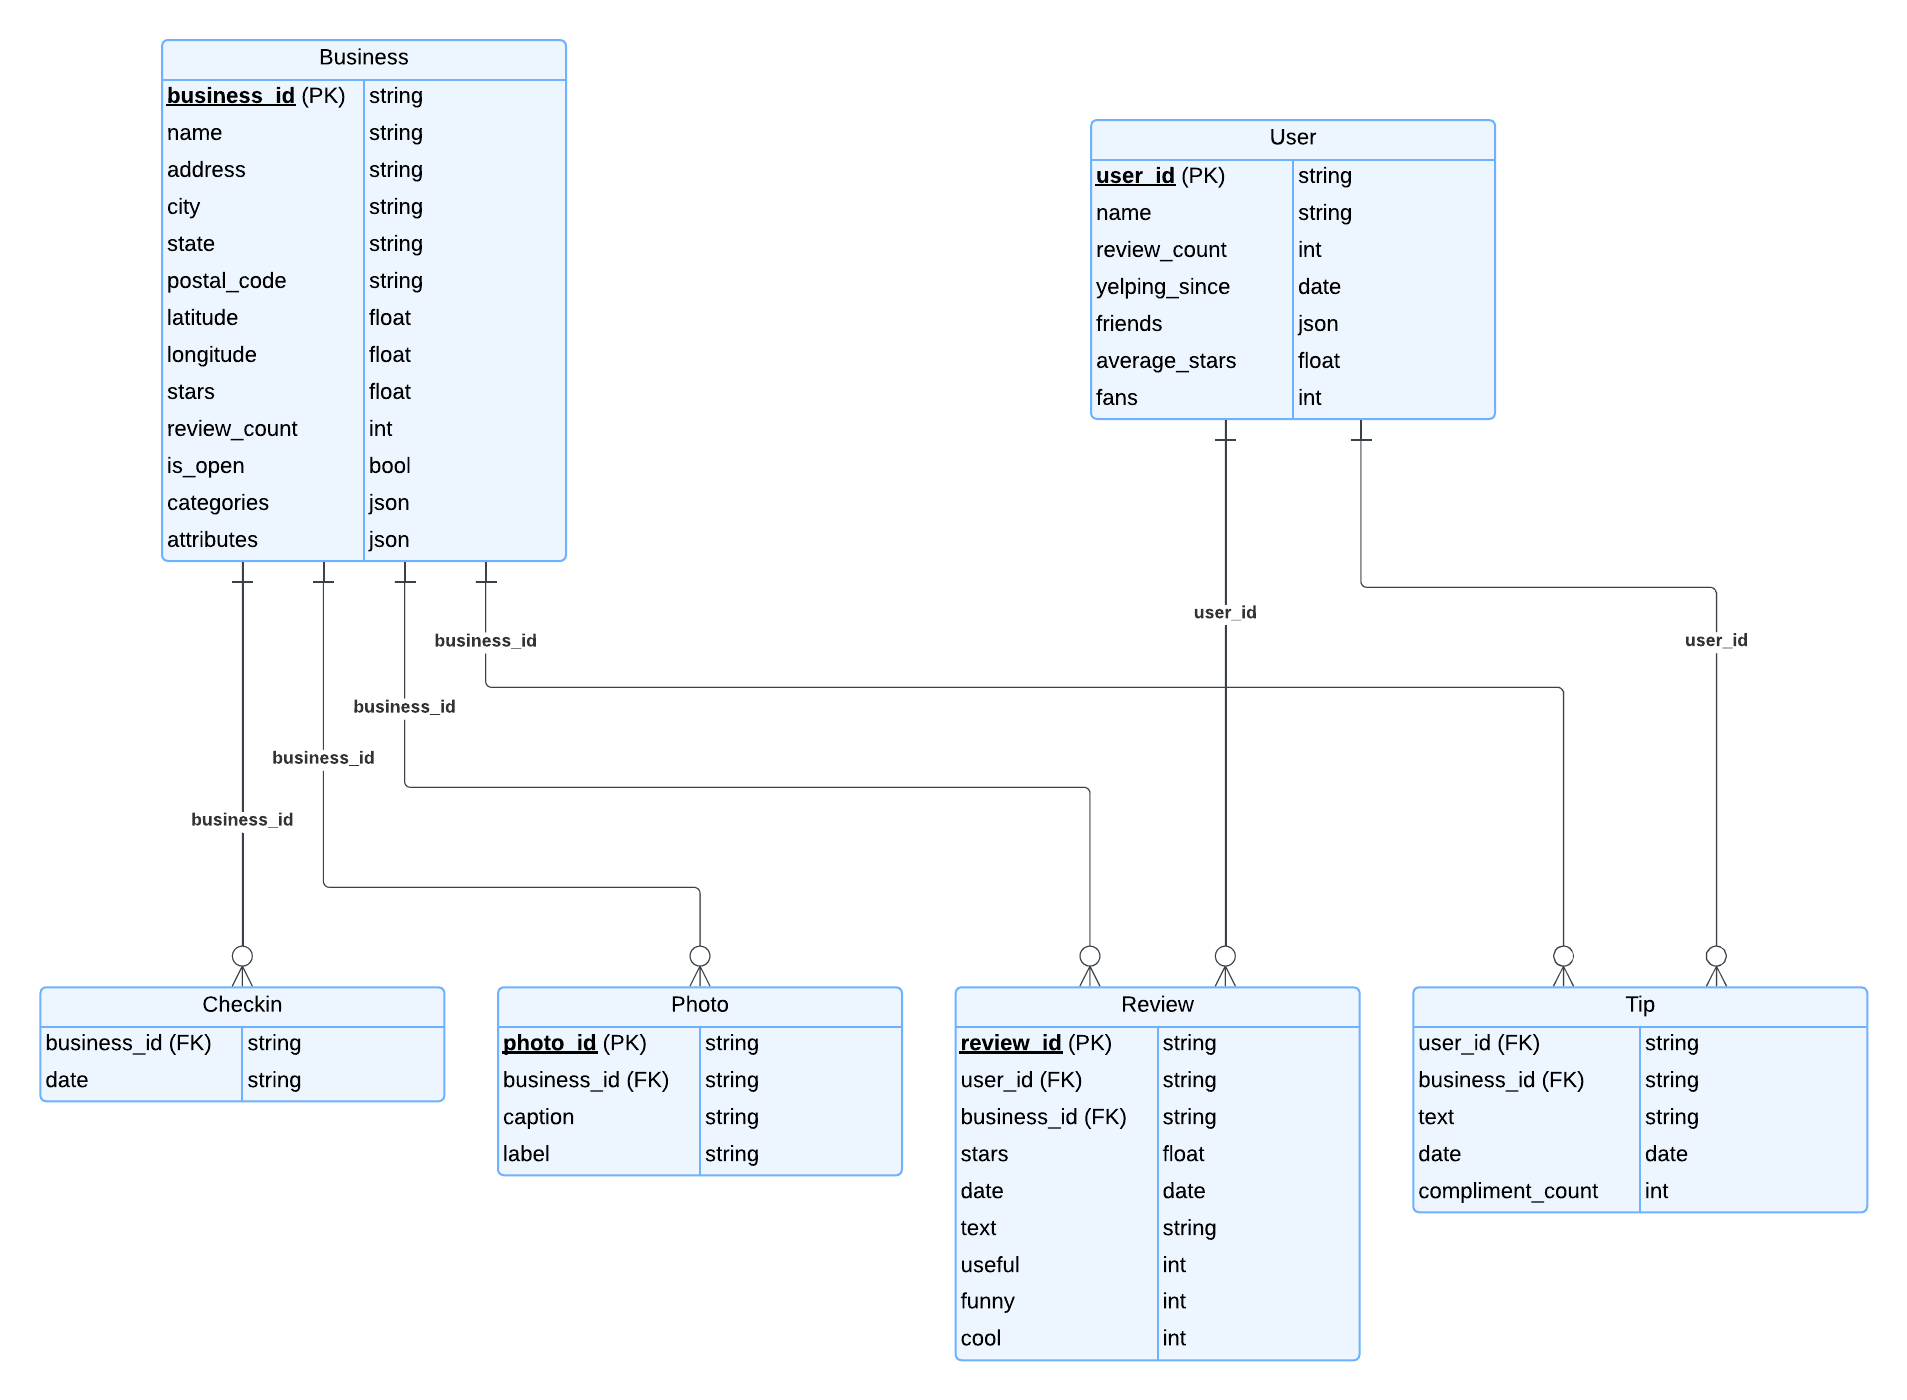
\includegraphics[width=0.8\textwidth]{er-diagram.png} % Change 'image.png' to your image file name
    \caption{ER diagram of Yelp dataset schema and relationships.}
    \label{fig:example} % Label for referencing the figure in the text
\end{figure}


As seen in our ER diagram, the dataset is made up of the following JSON files:
\begin{itemize}
    \item \textbf{business.json}: Business data, location data, attributes, and categories.
    \item \textbf{review.json}: Review text data, \texttt{user\_id} of the review writer, \texttt{business\_id} of the business reviewed, and review attributes and votes.
    \item \textbf{user.json}: User data, attributes, user friend mapping, user metadata.
    \item \textbf{checkin.json}: \texttt{business\_id}, date of check-in.
    \item \textbf{tip.json}: Tip text data, \texttt{user\_id} and \texttt{business\_id}.
    \item \textbf{photo.json}: Photo and \texttt{business\_ids}, photo attributes.
\end{itemize}

Each file is composed of a single object type, one JSON-object per line.


\section{Data Sampling and Truncation Plans}

The Yelp dataset is comprehensive, encompassing millions of records across users, businesses, and reviews. To ensure efficient processing while maintaining representativeness, we applied the following sampling and truncation strategies:

\begin{itemize}
    \item \textbf{Users:} The dataset originally contains several million user records. We sampled approximately 2 million users to reduce storage overhead and computational complexity. This sampling ensures proportional representation across different user activity levels and geographies.
    \item \textbf{Businesses:} All business records were retained without sampling. This allows for a complete representation of businesses across regions and categories.
    \item \textbf{Reviews:} Reviews were filtered based on references to existing users in the \texttt{users} table and businesses in the \texttt{businesses} table. This ensures referential integrity while excluding reviews that belong to users or businesses outside our database.
\end{itemize}

\section{Data Loading into PostgreSQL}



We used Python with the \texttt{psycopg} library to process and load the data into PostgreSQL. JSON data files were read line-by-line, parsed, and inserted into corresponding PostgreSQL tables. The loading process is summarized below:

\begin{itemize}
    \item \textbf{Schema Definition:} Tables for \texttt{users}, \texttt{businesses}, and \texttt{reviews} were defined with appropriate column types and constraints. Foreign key relationships were established to enforce referential integrity between \texttt{reviews} and the \texttt{users} and \texttt{businesses} tables.
    \item \textbf{Data Insertion:} For each table, the JSON data was parsed, and relevant fields were extracted. We used the \texttt{ON CONFLICT DO NOTHING} clause to handle duplicates and ensure the idempotency of the loading process.
    \item \textbf{Filtering for Referential Integrity:} Reviews referencing non-existent users or businesses were excluded during the loading process using SQL \texttt{JOIN}s and filters.
\end{itemize}

The SQL query used to retrieve the schema information is as follows:

\begin{lstlisting}[language=SQL, basicstyle=\ttfamily\small]
SELECT column_name, data_type
FROM information_schema.columns
WHERE table_name = 'business';
\end{lstlisting}

\subsubsection{Python Implementation}
The following Python code demonstrates the use of \texttt{psycopg} to connect to PostgreSQL and query the schema of the \texttt{business} table:

\begin{lstlisting}[language=Python, basicstyle=\ttfamily\small, breaklines=true]
import psycopg
import pandas as pd

# Connect to PostgreSQL
conn = psycopg.connect("dbname=yelp user=jadoo host=localhost")

# Query the schema of the business table
query = """
SELECT column_name, data_type
FROM information_schema.columns
WHERE table_name = 'business';
"""
schema_df = pd.read_sql(query, conn)
display(schema_df)
\end{lstlisting}

\subsubsection{Output of the Schema Query}
The schema for the \texttt{business} table is displayed below:

\begin{center}
\begin{tabular}{|c|c|}
\hline
\textbf{Column Name} & \textbf{Data Type} \\
\hline
hours & jsonb \\
latitude & double precision \\
longitude & double precision \\
stars & double precision \\
review\_count & integer \\
is\_open & integer \\
attributes & jsonb \\
business\_id & text \\
name & text \\
address & text \\
city & text \\
state & text \\
postal\_code & text \\
categories & text \\
\hline
\end{tabular}
\end{center}



\section{Query 1}

\subsection*{Problem}
Imagine we are working for Yelp, and they want to understand how many reviews the typical user posts.

\subsection*{Solution}
Our query provides a reasonable solution as it calculates the distribution of review counts per user by:
\begin{enumerate}
    \item Aggregating review counts for each user.
    \item Grouping these counts to show how many users fall into each category of review activity.
    \item Sorting the results for better visualization.
\end{enumerate}

\subsection*{SQL Query}
\begin{lstlisting}[caption={SQL Query to Analyze User Review Counts}, label={lst:user-review-counts}]
SELECT
    num_reviews,
    COUNT(*) AS num_users
FROM (
    SELECT
        r.user_id,
        COUNT(r.review_id) AS num_reviews
    FROM
        reviews r
    GROUP BY
        r.user_id
) AS user_review_counts
GROUP BY
    num_reviews
ORDER BY
    num_reviews DESC;
\end{lstlisting}


\begin{figure}[h!]
    \centering
    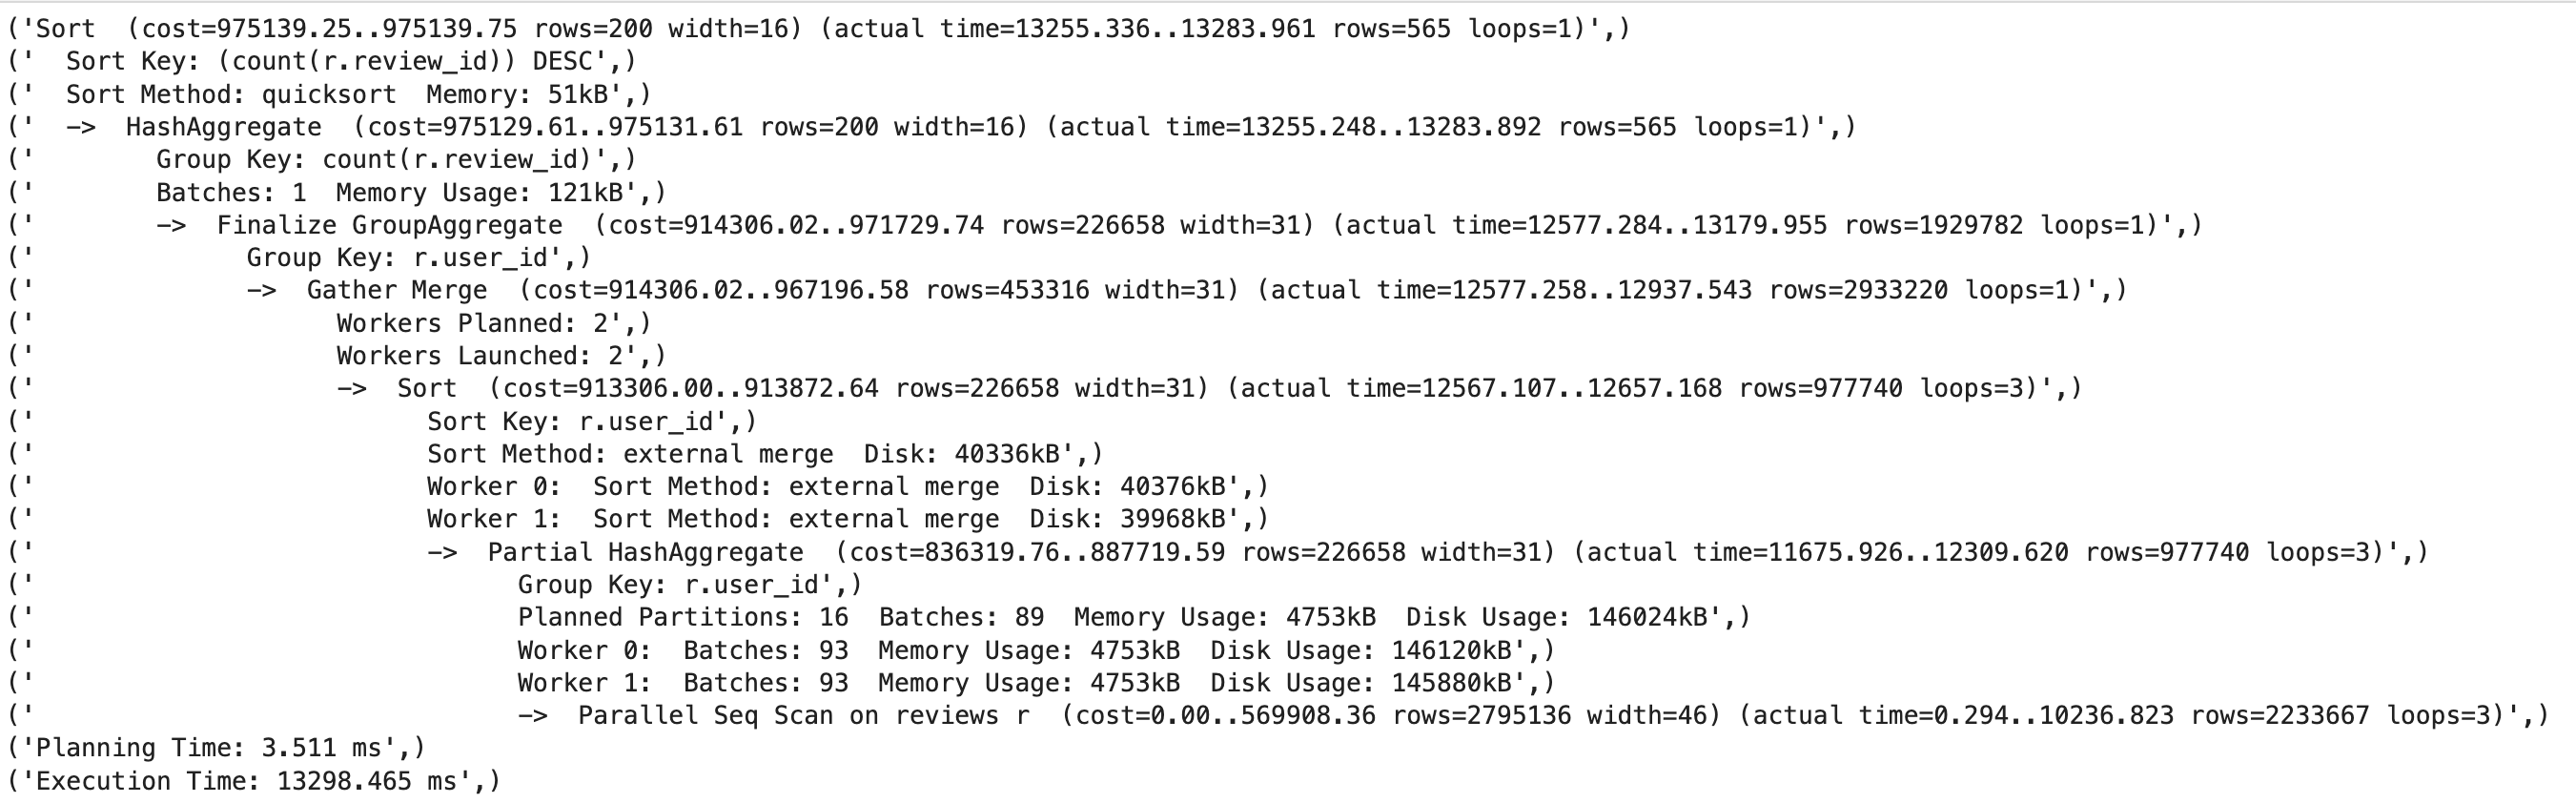
\includegraphics[width=0.8\textwidth]{correction.png} % Change 'image.png' to your image file name
    \caption{Distribution of Reviews per User}
    \label{fig:example} % Label for referencing the figure in the text
\end{figure}

The database setup and operations were performed on a local machine with 16GB RAM and SSD storage. PostgreSQL 14 was used as the relational database system. The entire dataset and the database are hosted locally to avoid network latency and ensure data privacy. JupyterLab was used for Python development and experimentation. 

This local setup provided the necessary computational resources and flexibility for our analysis.

\begin{figure}[h!]
    \centering
    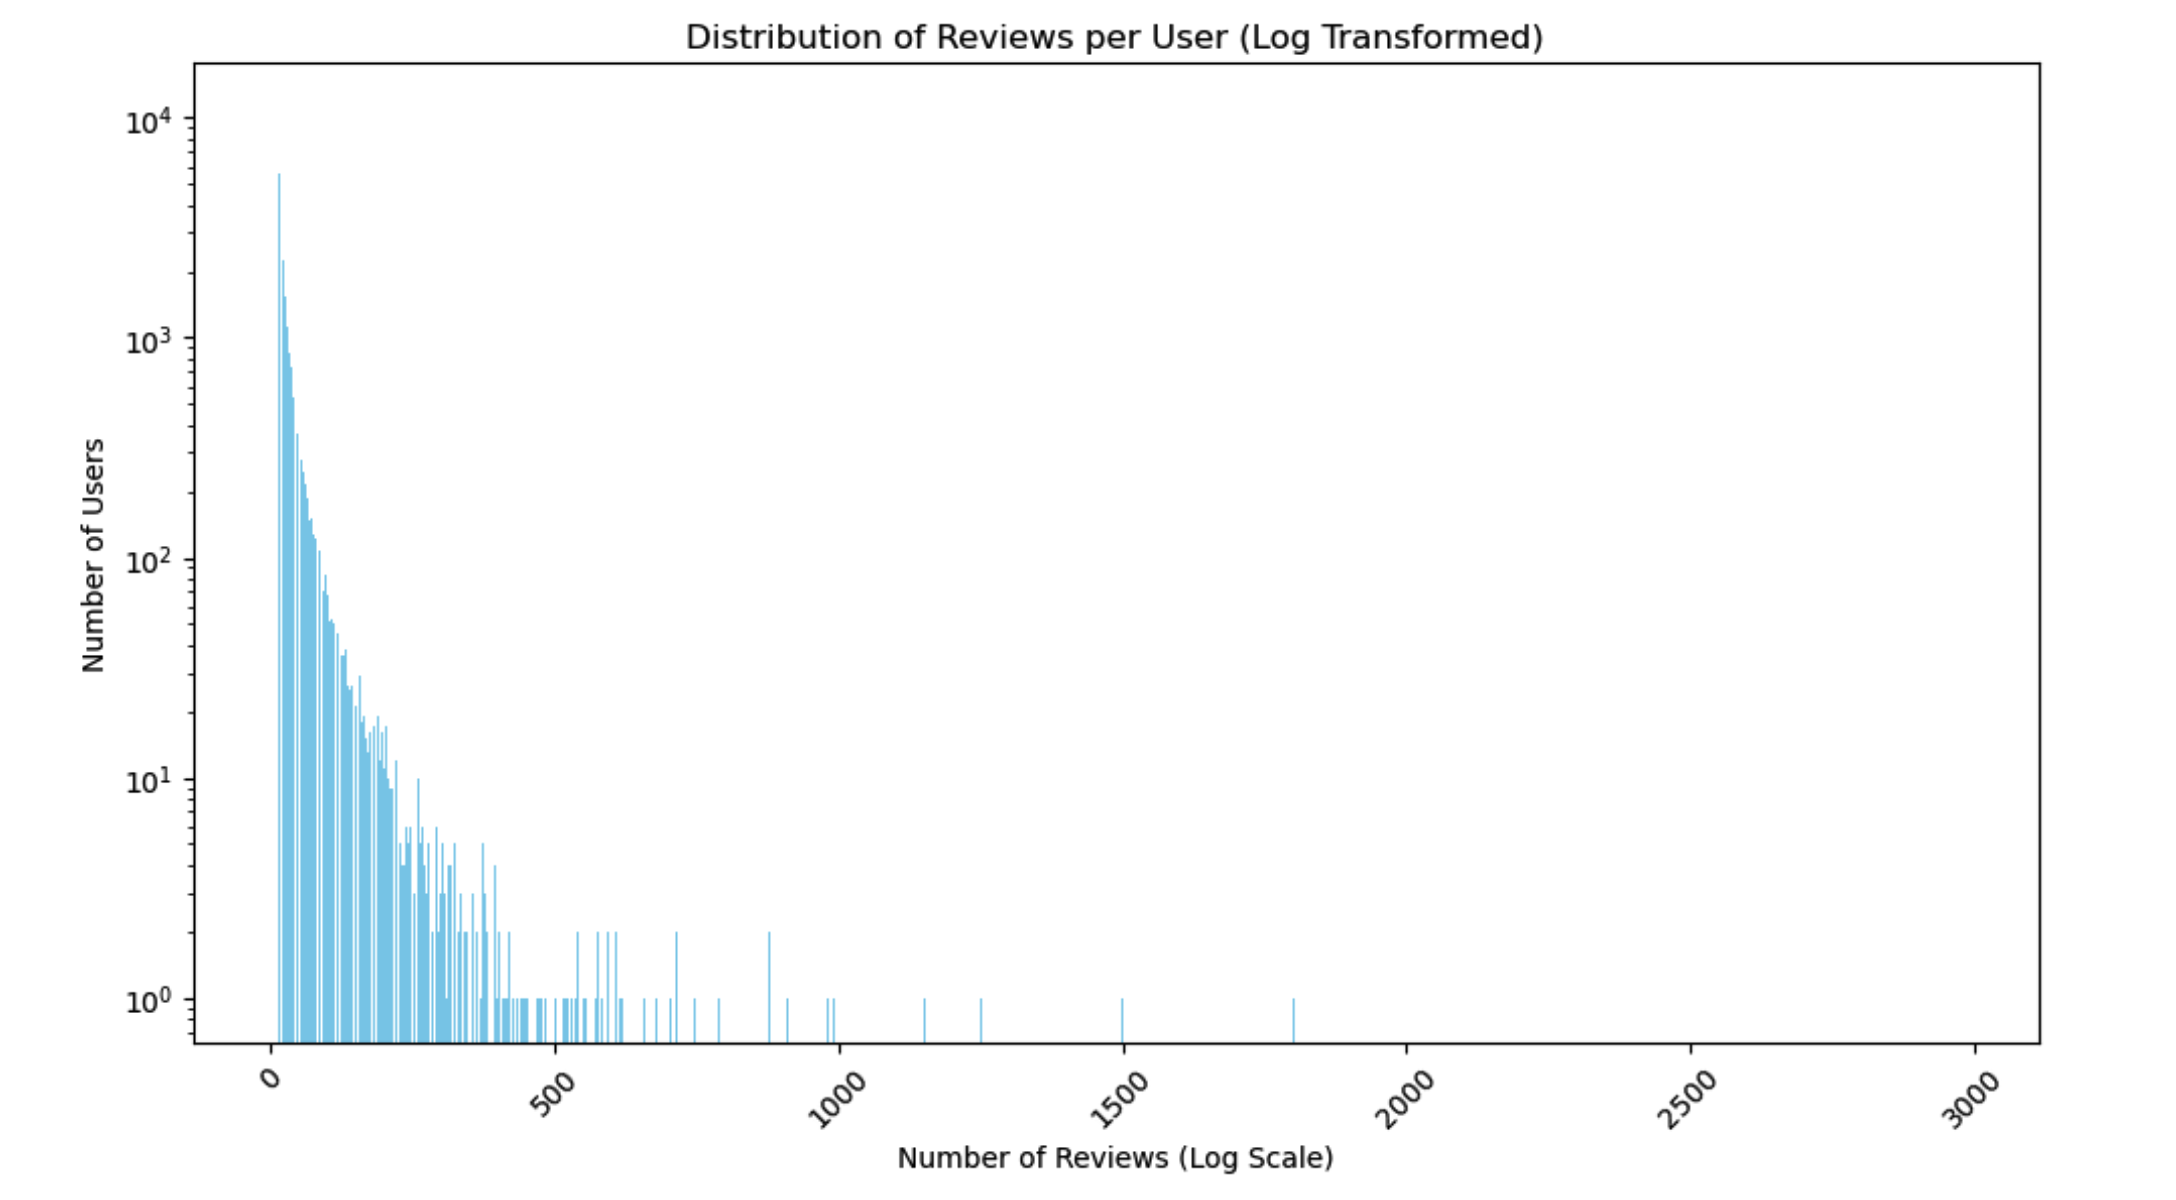
\includegraphics[width=0.8\textwidth]{graph.png} % Change 'image.png' to your image file name
    \caption{Distribution of Reviews per User}
    \label{fig:example} % Label for referencing the figure in the text
\end{figure}


\end{document}
